% Document settings
\documentclass[11pt]{article}
\usepackage{fancyhdr}
\usepackage[margin=1in]{geometry}
\usepackage[pdftex]{graphicx}
\usepackage{multirow}
\usepackage{setspace}
\pagestyle{plain}
\usepackage[american voltages]{circuitikz}
%\usepackage[american]{circuitikz}
\usepackage{graphicx}
\usepackage{multirow}
\usepackage{booktabs}
\usepackage{epstopdf}
%\usepackage{MnSymbol,wasysym}
\usepackage{amsmath}
%\usepackage{mathtools}
\usepackage{amssymb}
\usepackage{lipsum}
\usepackage{sympytex}
\usepackage{siunitx}
\setlength\parindent{0pt}
\graphicspath{{images/}{drawings/}}
% % % % % % % % % % % Header footer
% % % % % % % % % % %EDIT THIS % % % % % % % % % % % % % % % % % % % %
\pagestyle{fancy}
\fancyhf{}
\lhead{Tech Memo:  Experiment 1-Voltage Division}
\rhead{Andrei Tumbar}
\lfoot{EE281}
\cfoot{02/04/2020}
\rfoot{Page \thepage}
% % % % % % % % % % % % % % % % % % % % % % % % % % % % % % % % % % % % %


\begin{document}
	\numberwithin{equation}{subsection}
	\numberwithin{figure}{subsection}
	\hspace{6in}
		
\includegraphics[scale=0.9,trim=0cm 0in 0in 0.0in,clip]{RIT_KGCOE1}
\newline

\Huge \textbf{EEEE 281: Experiment 1 \\Voltage Division}\\

\Large
\textbf{From:} Andrei Tumbar [Computer Engineering] \\
\textbf{To: } Section 2 TA: LJ Boone, Harrison Keats \\
\textbf{Date: } Performed: 02/04/2020  Due: 02/11/2020 \\
\textbf{Subject: } Lab 1\\
\textbf{Lab Partner(s): } N/A\\
\vspace{0.5in}
	\begin{table}[h!]
		\centering
%		\caption{Grading Table}
		\label{Table:Grading Table 1}
		%\begin{tabular}{llllll}
		\begin{tabular}{|c||c|c|c|c|}
			\hline
			Component & Percentage of Grade   & Score \hspace{0.25in} & Comment \hspace{1in}  \\
			\hline
			Report Formatting & 20~\si{\percent} & & \\	 
			\hline 
			Hand Calculations: Circuit 1 & 10~\si{\percent} & & \\
			%Hand Calculations: Circuit 2 & 5~\si{\percent} & & \\
			\hline	
			PSPICE Setup: & 5~\si{\si{\percent}}&&\\
			\hline
			PSPICE Simulation:  & 10~\si{\percent} & & \\
			\hline
			PSPICE Discussion:  & 10~\si{\percent} & & \\
			%PSPICE Simulation: Circuit 2 & 10~\si{\percent} & & \\
			\hline
			Experimental Setup: & 5~\si{\percent} & & \\
			\hline
		    Experimental Data:  & 20~\si{\percent} & & \\	
		    %Experimental Data: Circuit 2 & 10~\si{\percent} & & \\	 
			\hline
			Experimental Discussion:  & 20~\si{\percent} & & \\	 
			\hline
			\textbf{Total Score:}&  & & \\	 
			\hline
			\textbf{Graded By:}&  & & \\	 
			\hline
			
		\end{tabular}
	\end{table}
\newpage
\Large \textbf{Abstract} \\
\normalsize
In the first part of this exercise, the software portion, a circuit with three resistors (two 5.6 k\si{\ohm}, 1 k\si{\ohm}) in series was designed in PSPICE, a circuit design, and simulation program. The resistors were listed with tolerances. A simulation was run to display a histogram of likely outcomes given the tolerance and resistance rating of each resistor. A Monte Carlo simulation displayed a statistical analysis of the likely outcomes of testing the circuit. In the hardware portion of the exercise, the circuit was implemented on a breadboard. The voltage was measured across each resistor given a supplied voltage of 5V. An effective resistance was measured along with resistance from each resistor. Finally, the voltage of each node relative to ground was measured and recorded. These experimentally determined values were compared to those calculated using the voltage division laws to analyze the circuit.

\section {Introduction and Theory}
The objective of this lab was to show how resistors in series will add overall resistance and show voltage division. Also, the Monte Carlo simulation showed how resistance tolerance can alter data.

\subsection{Theory: Circuits Investigated}

This circuit had a \(5\,V\) power source followed by two \(5.6\,k\si{\ohm}\) resistors followed by a \(1\,k\si{\ohm}\) resistor. The node between the final \(1\,k\si{\ohm}\) and the voltage source was grounded.

\begin{figure}[h!]
\begin{center}
\begin{circuitikz}
\draw
(0,4) to[battery, l_=5V] (0,0)
(0,4) to[R, -*, l_=\(R_1\,\text{$=$}\, 5.6\,k\si{\ohm}\), v^=$V_1$] (5,4) node[label={[font=\footnotesize]above:A}] {}
to[R, -*, l^=\(R_2\,\text{$=$}\, 5.6\,k\si{\ohm}\), v_=$V_2$] ++(5,0) node[label={[font=\footnotesize]above:B}] {}
to[R, l^=\(R_L\,\text{$=$}\, 1\,k\si{\ohm}\), v_=$V_L$] ++(0,-4)
-- ++(-5,0) node[ground]{} -- (0,0)
;
\end{circuitikz}
\end{center}
\caption{Circuit configuration given $R_1$, $R_2$, and $R_3$ with ground and voltage supply.}
\end{figure}

This is a simple series circuit with three resistors. The negative pole on the voltage supply is connected to ground. The voltage is set to $5\,V$. The first two resistors are both $5.6\,k\si\ohm$ resistors. The third resistor is a $1\,k\si\ohm$.

%\subsubsection{Theory: Equivalent Resistance}
%\begin{itemize}
%	\item Calculate the series resistance for each of the circuits as hand calculation. 
%	\item Include these calculations in a common equation such as Eqs.  \ref{Eq:ReqSeries} and \ref{Eq:ReqCircuit2}.  Rather than writing the equations as symbols, rewrite them with numbers and the final answer.
%	\begin{subequations}
%		\begin{equation}
%			\label{Eq:ReqSeries}
%			R_{eq,Circuit1}=R_1+R_2+R_L= SOLVE
%		\end{equation}
%		\begin{equation}
%		\label{Eq:ReqCircuit2}
%		R_{eq,Circuit2}=R_1+R_2+\left( R_L \parallel R_{L2} \right)=SOLVE
%		\end{equation}
%	\end{subequations}
%\end{itemize}

\subsubsection{Theory: Kirchhoff's Voltage Law and Voltage Division}
Kirchoff's Voltage law is the concept that the sum of the voltage drops in any loop equals zero. A loop is defined as a path where none of the nodes are visited more than once. The path must reach the original point. The idea of Voltage Divison states that in series, the voltage drop across each resistor is equal to the total voltage drop multiplied by the ratio of the current resistance to total resistance.

\begin{equation}
	\label{eq:1}
	V_1 = 5\,V \frac{5.6\,k\si\ohm}{5.6\,k\si\ohm + 5.6\,k\si\ohm + 1\,k\si\ohm} = 2.295\,V
\end{equation}
\begin{equation}
	\label{eq:2}
	V_2 = 5\,V \frac{5.6\,k\si\ohm}{5.6\,k\si\ohm + 5.6\,k\si\ohm + 1\,k\si\ohm} = 2.295\,V
\end{equation}
\begin{equation}
	\label{eq:3}
	V_L = 5\,V \frac{1\,k\si\ohm}{5.6\,k\si\ohm + 5.6\,k\si\ohm + 1\,k\si\ohm} = 0.410\,V
\end{equation}

$V_A$ can be found by moving from the bottom node connected to ground to the node labeled $A$. There is a $5\,V$ gain from the voltage source, then there is a $2.295\,V$ drop across $R_1$. Therefore the voltage $V_A$ is $2.705$ relative to ground. The same method was used to find the voltage $V_B$ which evaluated to be $0.410\,V$.

%\subsubsection{Theory: Kirchhoff's Current Law and Current Division}
%In this section, you should briefly introduce the reader to the concepts of Kirchhoff's Current Law and Current Division.  You do NOT need to derive expressions for each here. 
%	\begin{itemize}
%		\item Determine the current through each branch of Circuit 2.  Show that Kirchhoff's Current Law holds. 
%		\item You will need to determine the current leaving the voltage supply (one sentence and corresponding equation).
%		\item Next use current division to determine the current through each of the load resistors via current division (one sentence, two equations)
%	\end{itemize}
%\subsubsection{Theory: Power Balance}
%In this section, you should briefly introduce the reader to the concepts of conservation of power. For each circuit:
%\begin{itemize}
%	\item Determine the power absorbed by each circuit element and show that the net sum of powers=0. 
%	\item There should be one equation for each circuit, and a brief summary.  
%\end{itemize}
\subsection{Theory: PSPICE Simulation Summary}
%Begin by providing a 1 paragraph description of the PSPICE setup. Was a DC simulation used, transient simulation, etc.?  Which \textbf{libraries} and \textbf{PSPICE elements} were used in the simulation? As you develop your lab reports this term, aspects of this text may be applicable in future reports.  In order to determine the libraries used, you can find the information when you look at the properties of each element.  There will be a reference to a ``.olb'' file.  This is the library name.   Look to the Appendix in Prof. Rommel's PSPICE tutorial if you are not sure as to the names/nomenclature.  For example, the resistors used are ``R/ANALOG'' from the \textbf{analog.olb} library. 

The PSPICE simulation began with a design of the circuit. A voltage supply along with three resistors were placed. A $10\percent$ tolerance was added to each of the resistors. The resistance was set for each element. The nodes $A$ and $B$ were named as such. A ground was placed according to the circuit diagram in figure. The PSPICE setup used the libraries imported from the Circuits 1 library from the lab computer. The libraries were called \textbf{analog.olb}, \textbf{opamp.olb}, \textbf{source.olb}, and \textbf{special.olb}. The components used were ``R/ANALOG'' from the \textbf{analog.olb} for the resistors, ``VDC/SOURCE'' from the \textbf{source.olb} for the voltage source and ``O/CAPSYM'' from the \textbf{special.olb} for ground.

\subsubsection{PSPICE: DC Simulation of Circuit 1}

\begin{figure}[htbp]
	\centering
	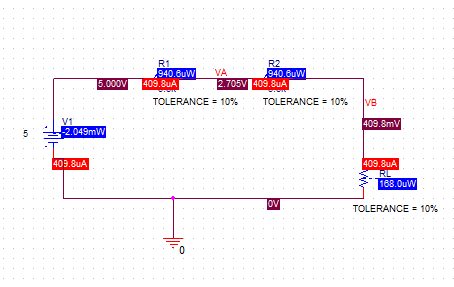
\includegraphics[height=10cm]{schematic}
	\caption{Circuit 1 with voltage markers.}
	\label{Fig:Circuit1VoltageMarkers}
\end{figure}

\begin{table}[h!]
	\caption{Simulation results for Circuit 1.}
	\begin{center}
		\begin{tabular}{|c||c|}
			\hline
			Node & Voltage (\si{\volt}) \\
			\hline
			Supply & 5 \\	 
			\hline 
			Node A & 2.708 \\	 
			\hline
			Node B & 0.411 \\	 
			\hline			
		\end{tabular}
	\end{center}
	\label{Table: Circuit 1}
\end{table}	

The results in Table \ref{Table: Circuit 1} agree with the hand calculations in equations \ref{eq:1}\,-\,\ref{eq:3}.

\subsubsection{PSPICE: Monte Carlo Simulation for Circuit 1}

\begin{figure}[htbp]
	\centering
	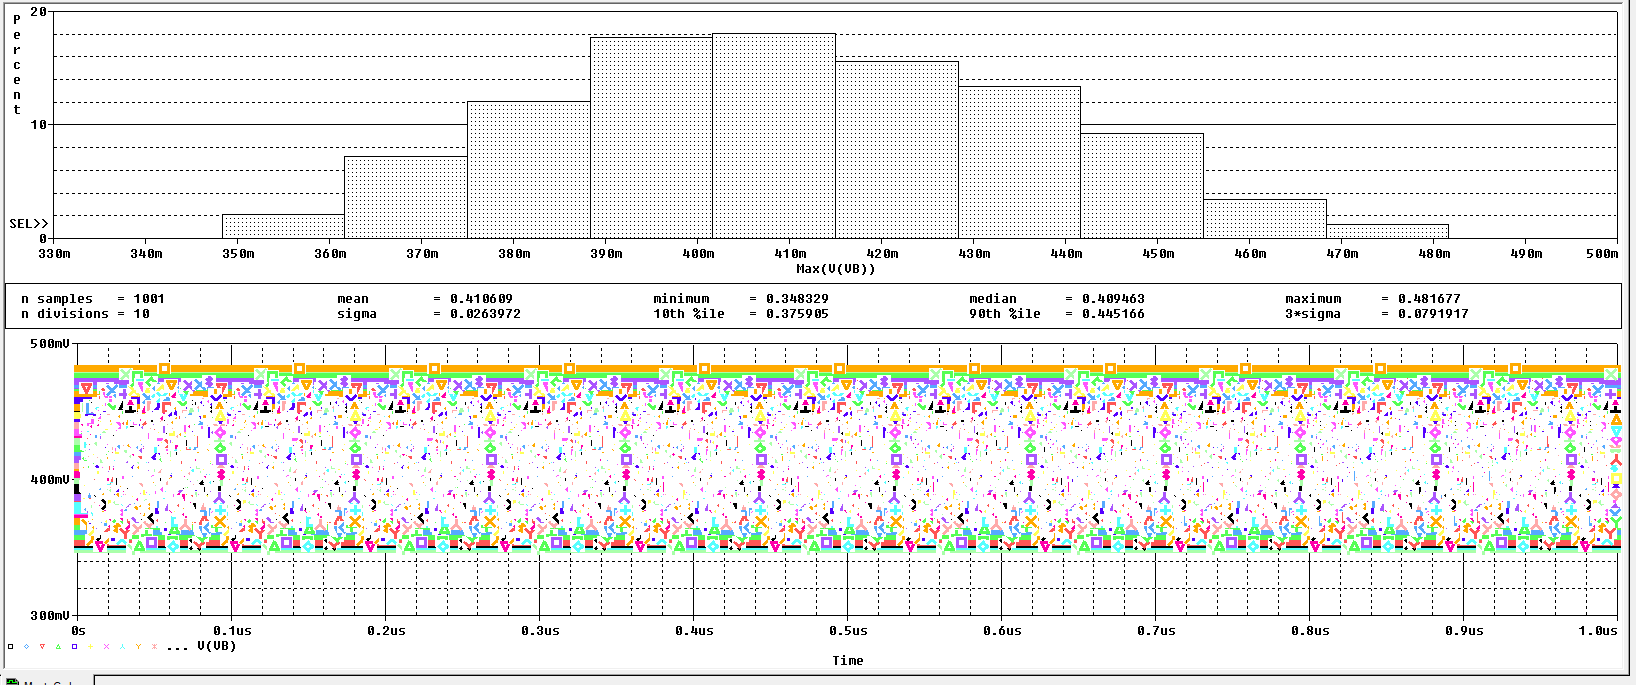
\includegraphics[width=\textwidth]{simulation}
	\caption{Monte Carlo simulation of Circuit 1.}
	\label{Fig:Circuit1MonteCarlo}
\end{figure}

The Monte Carlo simulation shown in \ref{Fig:Circuit1MonteCarlo} shows a probalility curve for likely measurements from Circuit 1. The highest probalility can be seen in the highest column at around $0.407\,\si\volt$ This is very close to the calculated value of $0.410\,\si\volt$. The bars around the center show other likely measurements based on the tolerance set. The mean value found through the Monte Carlo simulation was $0.411\,\si\volt$ and the sigma was $0.026$. 

\section{Hardware Experiment: Results and Discussion}
The circuit board was set up by connecting the power rail on the board to the 6V source on the DC power supply. The positive terminal on the rail was connected to the first $5.6\,k\si\ohm$ resistor. This first resistor was then put in series with the second $5.6\,k\si\ohm$ resistor and finally the $1\,k\si\ohm$ resistor. The node after the $1\,k\si\ohm$ resistor was connected to the negative terminal on the power rail. \par

The power supply was configured to $5\,\si\volt$ and the current was limited to $0.1\,\si\ampere$. This was done to prevent overheating in the case of a short circuit.

\pagebreak

\subsection{Equipment Used in the Laboratory}
%Write a short paragraph to detail the equipment used in the laboratory, and specific model numbers. Ideally, you should create a table of the equipment which should be referred to in text (See Table \ref{Table:Equipment} as an example).  The room location where the experiment was performed should be included.  Note that this should be a part of all Tech Memos, as it is an essential piece for other users to replicate your experiment.  \textbf{As you will be likely using the same equipment throughout the term, once the text/tables are established, you may reuse the information with the permission of your instructor/TA.}

\begin{table}[htbp]
	\setlength{\tabcolsep}{14pt}
	\centering
	\caption{Equipment/Software required for Lab 1.}
	\label{Table:Equipment}
	%\begin{tabular}{llllll}
	\begin{tabular}{|c||c|c|c|c|}
		\hline
		Item & Tool & Room      \\
		\hline
		Simulation & OrCAD Capture CIS & 09-3200   \\
		\hline  
		DC Power Supply & Agilent E3631A   & 09-3200 \\ 
		\hline 
		Multimeter & Agilent 34401A & 09-3200 \\
		\hline
		%				Oscilloscope & Textronix TDS2012C & 09-3200  \\
		%				\hline
		%				Oscilloscope & Agilent DSO 33120A & 09-3170  \\
		%				\hline
		%				
	\end{tabular}
\end{table}

OrCAD was used to create the circuit and the perform the Monte Carlo simulation. The DC Power Supply shows in Table \ref{Table:Equipment} was used in the hardware portion to power the circuit. The multimeter shown was used to measure the voltage and resistances across each of the resistors.

\subsection{Hardware Results/Discussion Circuit 1}	
%At least a paragraph should be included here to discuss the results. Some points to include are listed below:



%\begin{itemize}
%	\item Present the nodal voltages measured in Table \ref{Table:ResultsCircuit1}.
%	\item Present the differential voltages measured in Table \ref{Table:DerivedResultsCircuit1}.  %Use Ohm's law as we did in the laboratory to complete the table.

%	\item Kirchhoff's Voltage Law (sum of all voltages around a closed loop=0) is satisfied.   Provide a simple calculation to back this up.
%	\item Power conservation (sum of all powers around a closed loop = 0) is satisfied.
%	\item Compare the measured result to the PSPICE for the \textbf{nodal voltages} reported in Table \ref{Table:ResultsCircuit1}. Perform an error analysis and report the data in the table.
%\end{itemize}

The low error from PSPICE indicate that the resistors did not vary too far from the listed resistances. The Node B voltage had the highest error because that resistor had the lowest value. Therefore the likelihood of error is higher than the other two.

\begin{equation}
\label{eq:error}
E_{percent} = \frac{|V_{pspice} - V_{measured}|}{V_{pspice}}
\end{equation}

Equation \ref{eq:error} was used to calculate the error each of the measured voltages in Table \ref{Table:ResultsCircuit1}.

\begin{table}[h!]
	\caption{Experimental nodal voltages for Circuit 1.}
	%\begin{tabular}{llllll}
	\begin{center}
		\begin{tabular}{|c||c|c|c|}
			\hline
		Node & Voltage (\si{\volt}) & Percent Error With PSPICE \\
		\hline
		Supply & 5.002 & $0.04 \percent$\\	 
		\hline 
		Node A & 2.708 & $0.1\percent$\\	 
		\hline
		Node B & 0.405 & $1.5\percent$\\	 
		\hline			
		\end{tabular}
	\end{center}
	\label{Table:ResultsCircuit1}
\end{table}

\begin{table}[h!]
	\caption{Differential voltages and measured resistances for Circuit 1.}
	\label{Table:DerivedResultsCircuit1}
	%\begin{tabular}{llllll}
	\begin{center}
		\begin{tabular}{|c||c|c|c|c|c|}
			\hline
			Element & Component & Measured & Voltage  \\
			& Value & Resistance (\si{\ohm}) & (\si{\volt})     \\
	
			\hline
			Supply & 5~\si{\volt} & N/A & 5.002 \\	 
			\hline 
			$R_1$ & 5600~\si{\ohm} & 5560 & 2.292 \\	 
			\hline
			$R_2$ & 5600~\si{\ohm} & 5576 & 2.303 \\
			\hline
			$R_L$ & 1000~\si{\ohm} & 1005 & 0.405 \\
			\hline
		\end{tabular}
	\end{center}
\end{table}

When Kirchoff's Voltage Law is applied to the measured value, the following is observered:

\begin{equation}
\label{eq:kirchoff}
2.292\,\si\volt + 2.303\,\si\volt + 0.405\,\si\volt - 5.002\,\si\volt = -0.002\,\si\volt
\end{equation}

Equation \ref{eq:kirchoff} shows that Kirchoff's Voltage law holds for this circuit.

%\subsection{Hardware Results/Discsussion Circuit 2}	
% At least a paragraph should be included here to discuss the results. Some points to include are listed below:
%\begin{itemize}
%	\item Present the nodal voltages measured in Table \ref{Table:ResultsCircuit2}.
%	\begin{table}[h!]
%		\centering
%		\caption{Experimental nodal voltages for Circuit 2.}
%		\label{Table:ResultsCircuit2}
%		%\begin{tabular}{llllll}
%		\begin{tabular}{|c||c|c|c|}
%			\hline
%			Node & Voltage (\si{\volt}) & Percent Error (Hand Calc.) & Percent Error (PSPICE) \\
%			\hline
%			Supply & & &\\	 
%			\hline 
%			Node A &  & &\\	 
%			\hline
%			Node B &  &  &\\	 
%			\hline				
%		\end{tabular}
%	\end{table}
%	
%	\item Present the differential voltages measured in Table \ref{Table:DerivedResultsCircuit2}.  Use Ohm's law as we did in the laboratory to complete the table.
%			\begin{table}[h!]
%				\centering
%				\caption{Derived Results for Circuit 2.}
%				\label{Table:DerivedResultsCircuit2}
%				%\begin{tabular}{llllll}
%				\begin{tabular}{|c||c|c|c|c|c|}
%					\hline
%					Element & Component & Measured & Voltage & Current & Power \\
%					& Value & Resistance (\si{\ohm}) & (\si{\volt}) & (\si{\ampere}) &  
%					(\si{\watt})    \\
%					\hline
%					Supply & 5~\si{\volt} & N/A & & &\\	 
%					\hline 
%					$R_1$ & 1000~\si{\ohm} & & & &\\	 
%					\hline
%					$R_2$ & 1000~\si{\ohm}& & & &\\	 
%					\hline
%					$R_L$ & 1000~\si{\ohm} & & & &\\	 
%					\hline
%					$R_{L2}$ & 180~\si{\ohm} & & & &\\	 
%					\hline				
%				\end{tabular}
%			\end{table}
%\end{itemize}
%For this circuit, in your report you should demonstrate: 
%\begin{itemize}
%	\item Kirchhoff's Voltage Law (sum of all voltages around a closed loop=0) is satisfied.   Do this for all closed loops in the circuit.  Provide a simple calculation to back this up.
%	\item Power conservation (sum of all powers around a closed loop = 0) is satisfied. Do this for all closed loops in the circuit.
%	\item Kirchhoff's Current Law (sum of currents entering a node is equal to 0) is satisfied. Show that current division can be used to explain the splitting of currents between $R_L$ and $R_{L2}$.
%	\item Compare the measured result to the PSPICE and theoretical calculations for the \textbf{nodal voltages} reported in Table \ref{Table:ResultsCircuit2}. Perform an error analysis and report the data in the table.
%\end{itemize}

\pagebreak

\section{Conclusion}
%	Provide a 1 paragraph summary of the laboratory experiment.  What were the major conclusions for each circuit topology?  Also did the theory agree with the experiment?  The conclusion is a revised version of the abstract.

The purpose of this exercise was to show the use of voltage division and kirchoff's law as well as show error analysis with PSPICE. A circuit was designed with three resistors in series and run through a Monte Carlo simulation to show likely measurements. The circuit was then built on a breadboard and measurements were compared to PSPICE. Percent error was analysed to be within the tolerance rated on the resistor.
	
	\section{Acknowledgments}
	\begin{itemize}
	\item Petre Tumbar helped through the PSPICE Monte Carlo setup.
	\item wikibooks.org helped with the \LaTeX\;code.
	\end{itemize}
	
\begin{thebibliography}{9}
	\bibitem{AlexanderSadiku}
	C.K. Alexander, and M.K.O. Sadiku,
	\emph{Fundamentals of Electric Circuits, 4th Edition},
	McGraw Hill, pp. xx-yy(EDIT), 2009.
	\bibitem{RommelLab}
	S. Rommel,
	\emph{EEEE 281 Lab 1 Lecture notes}, Spring 2015.
\end{thebibliography}

\end{document}



